\documentclass{beamer}
\usepackage{graphicx}
\usepackage{listings}
\usepackage{amsfonts}
\usepackage{amsmath}
\usepackage{multicol}
\usepackage[pdf]{graphviz}
\usepackage[skins,breakable,listings]{tcolorbox}

\lstset{basicstyle=\ttfamily,breaklines=true}
\usepackage{upquote}
%\def\backtick{\char18}
\lstdefinestyle{backtickstyle}{literate={`}{\char}1, escapechar=@}

\usepackage{fontspec}

\makeatletter
\def\verbatim@nolig@list{}
\makeatother

\setmonofont{JetBrains Mono}[Contextuals=Alternate]

\usepackage{ocr}
\usepackage[T1]{fontenc}

\usepackage{accsupp}
\newcommand{\noncopyable}[1]{%
\BeginAccSupp{method=escape,ActualText={}}%
#1%
\EndAccSupp{}%
}

\lstdefinelanguage{kotlin}{
comment=[l]{//},
commentstyle={\color{gray}\ttfamily},
emph={delegate, filter, firstOrNull, forEach, it, lazy, mapNotNull, println, repeat, assert, with, head, tail, len, return@},
numberstyle=\noncopyable,
emphstyle={\color{olive}},
identifierstyle=\color{black},
keywords={abstract, actual, as, as?, break, by, class, companion, continue, data, do, dynamic, else, enum, expect, false, final, for, fun, get, if, import, in, infix, interface, internal, is, null, object, open, operator, override, package, private, public, return, sealed, set, super, suspend, this, throw, true, try, catch, typealias, val, var, vararg, when, where, while, tailrec, reified, Repeat},
keywordstyle={\color{blue}\bfseries},
morecomment=[s]{/*}{*/},
morestring=[b]",
morestring=[s]{"""*}{*"""},
ndkeywords={@Deprecated, @JvmField, @JvmName, @JvmOverloads, @JvmStatic, @JvmSynthetic, Array, Byte, Double, Float, Boolean, Int, Integer, Iterable, Long, Runnable, Short, String, Pair},
ndkeywordstyle={\color{purple}\bfseries},
sensitive=true,
stringstyle={\color{green}\ttfamily},
literate={`}{{\char0}}1
}

\newtcblisting{kotlinlisting}[1][]{%
listing options={
language=kotlin,
basicstyle=\scriptsize\ttfamily,
%numberstyle=\footnotesize\noncopyable,
showstringspaces=false,
tabsize=2,
breaklines=true,
%numbers=right,
inputencoding=utf8,
escapeinside={(*@}{@*)},
#1
},
underlay unbroken and first={%
\path[draw=none] (interior.north west) rectangle node[white]{
\includegraphics[width=4mm]{../figures/kotlin_file.png}} ([xshift=-10mm,yshift=-12mm]interior.north west);
}
}

\tcbset{
enhanced jigsaw,
listing only,
%boxsep=-1pt,
%top=-1pt,
%bottom=-0.5pt,
center,
width=0.92\textwidth,
%right=-0.5pt,
overlay first={
\node[black!50] (S) at (frame.south) {\Large\ding{34}};
\draw[dashed,black!50] (frame.south west) -- (S) -- (frame.south east);
},
overlay middle={
\node[black!50] (S) at (frame.south) {\Large\ding{34}};
\draw[dashed,black!50] (frame.south west) -- (S) -- (frame.south east);
\node[black!50] (S) at (frame.north) {\Large\ding{34}};
\draw[dashed,black!50] (frame.north west) -- (S) -- (frame.north east);
},
overlay last={
\node[black!50] (S) at (frame.north) {\Large\ding{34}};
\draw[dashed,black!50] (frame.north west) -- (S) -- (frame.north east);
},
before={\par\vspace{10pt}},
after={\par\vspace{10pt}\noindent}
}

\newcommand*{\inlineimg}[1]{%
\raisebox{-.3\baselineskip}{%
\includegraphics[
height=\baselineskip,
width=\baselineskip,
keepaspectratio,
]{#1}%
}%
}

\definecolor{slightgray}{rgb}{0.90, 0.90, 0.90}

\usepackage{soul}
\usepackage{hyperref}
\makeatletter
\def\SOUL@hlpreamble{%
\setul{}{3.0ex}%
\let\SOUL@stcolor\SOUL@hlcolor%
\SOUL@stpreamble%
}
\makeatother

\newcommand{\inline}[1]{%
\begingroup%
\sethlcolor{slightgray}%
\hl{\ttfamily\footnotesize #1}%
\endgroup
}

\newcommand{\tinline}[1]{%
\begingroup%
\sethlcolor{slightgray}%
\hl{\ttfamily\tiny #1}%
\endgroup
}

\mode<presentation> { \usetheme{Madrid} }

\title{Concepts in Statistical and Software Testing}
\subtitle{COMP 598, Recitation \#2}

\author{Breandan Considine}

\institute[McGill]{
McGill University \\
\medskip
\textit{breandan.considine@mcgill.ca}
}
\date{\today}


\begin{document}
\begin{frame}
    \titlepage
\end{frame}

%\begin{frame}
%    \frametitle{Overview}
%    \tableofcontents
%\end{frame}

\section{Traditional Software Engineering}

\begin{frame}
\frametitle{Royce's Waterfall Model}
\center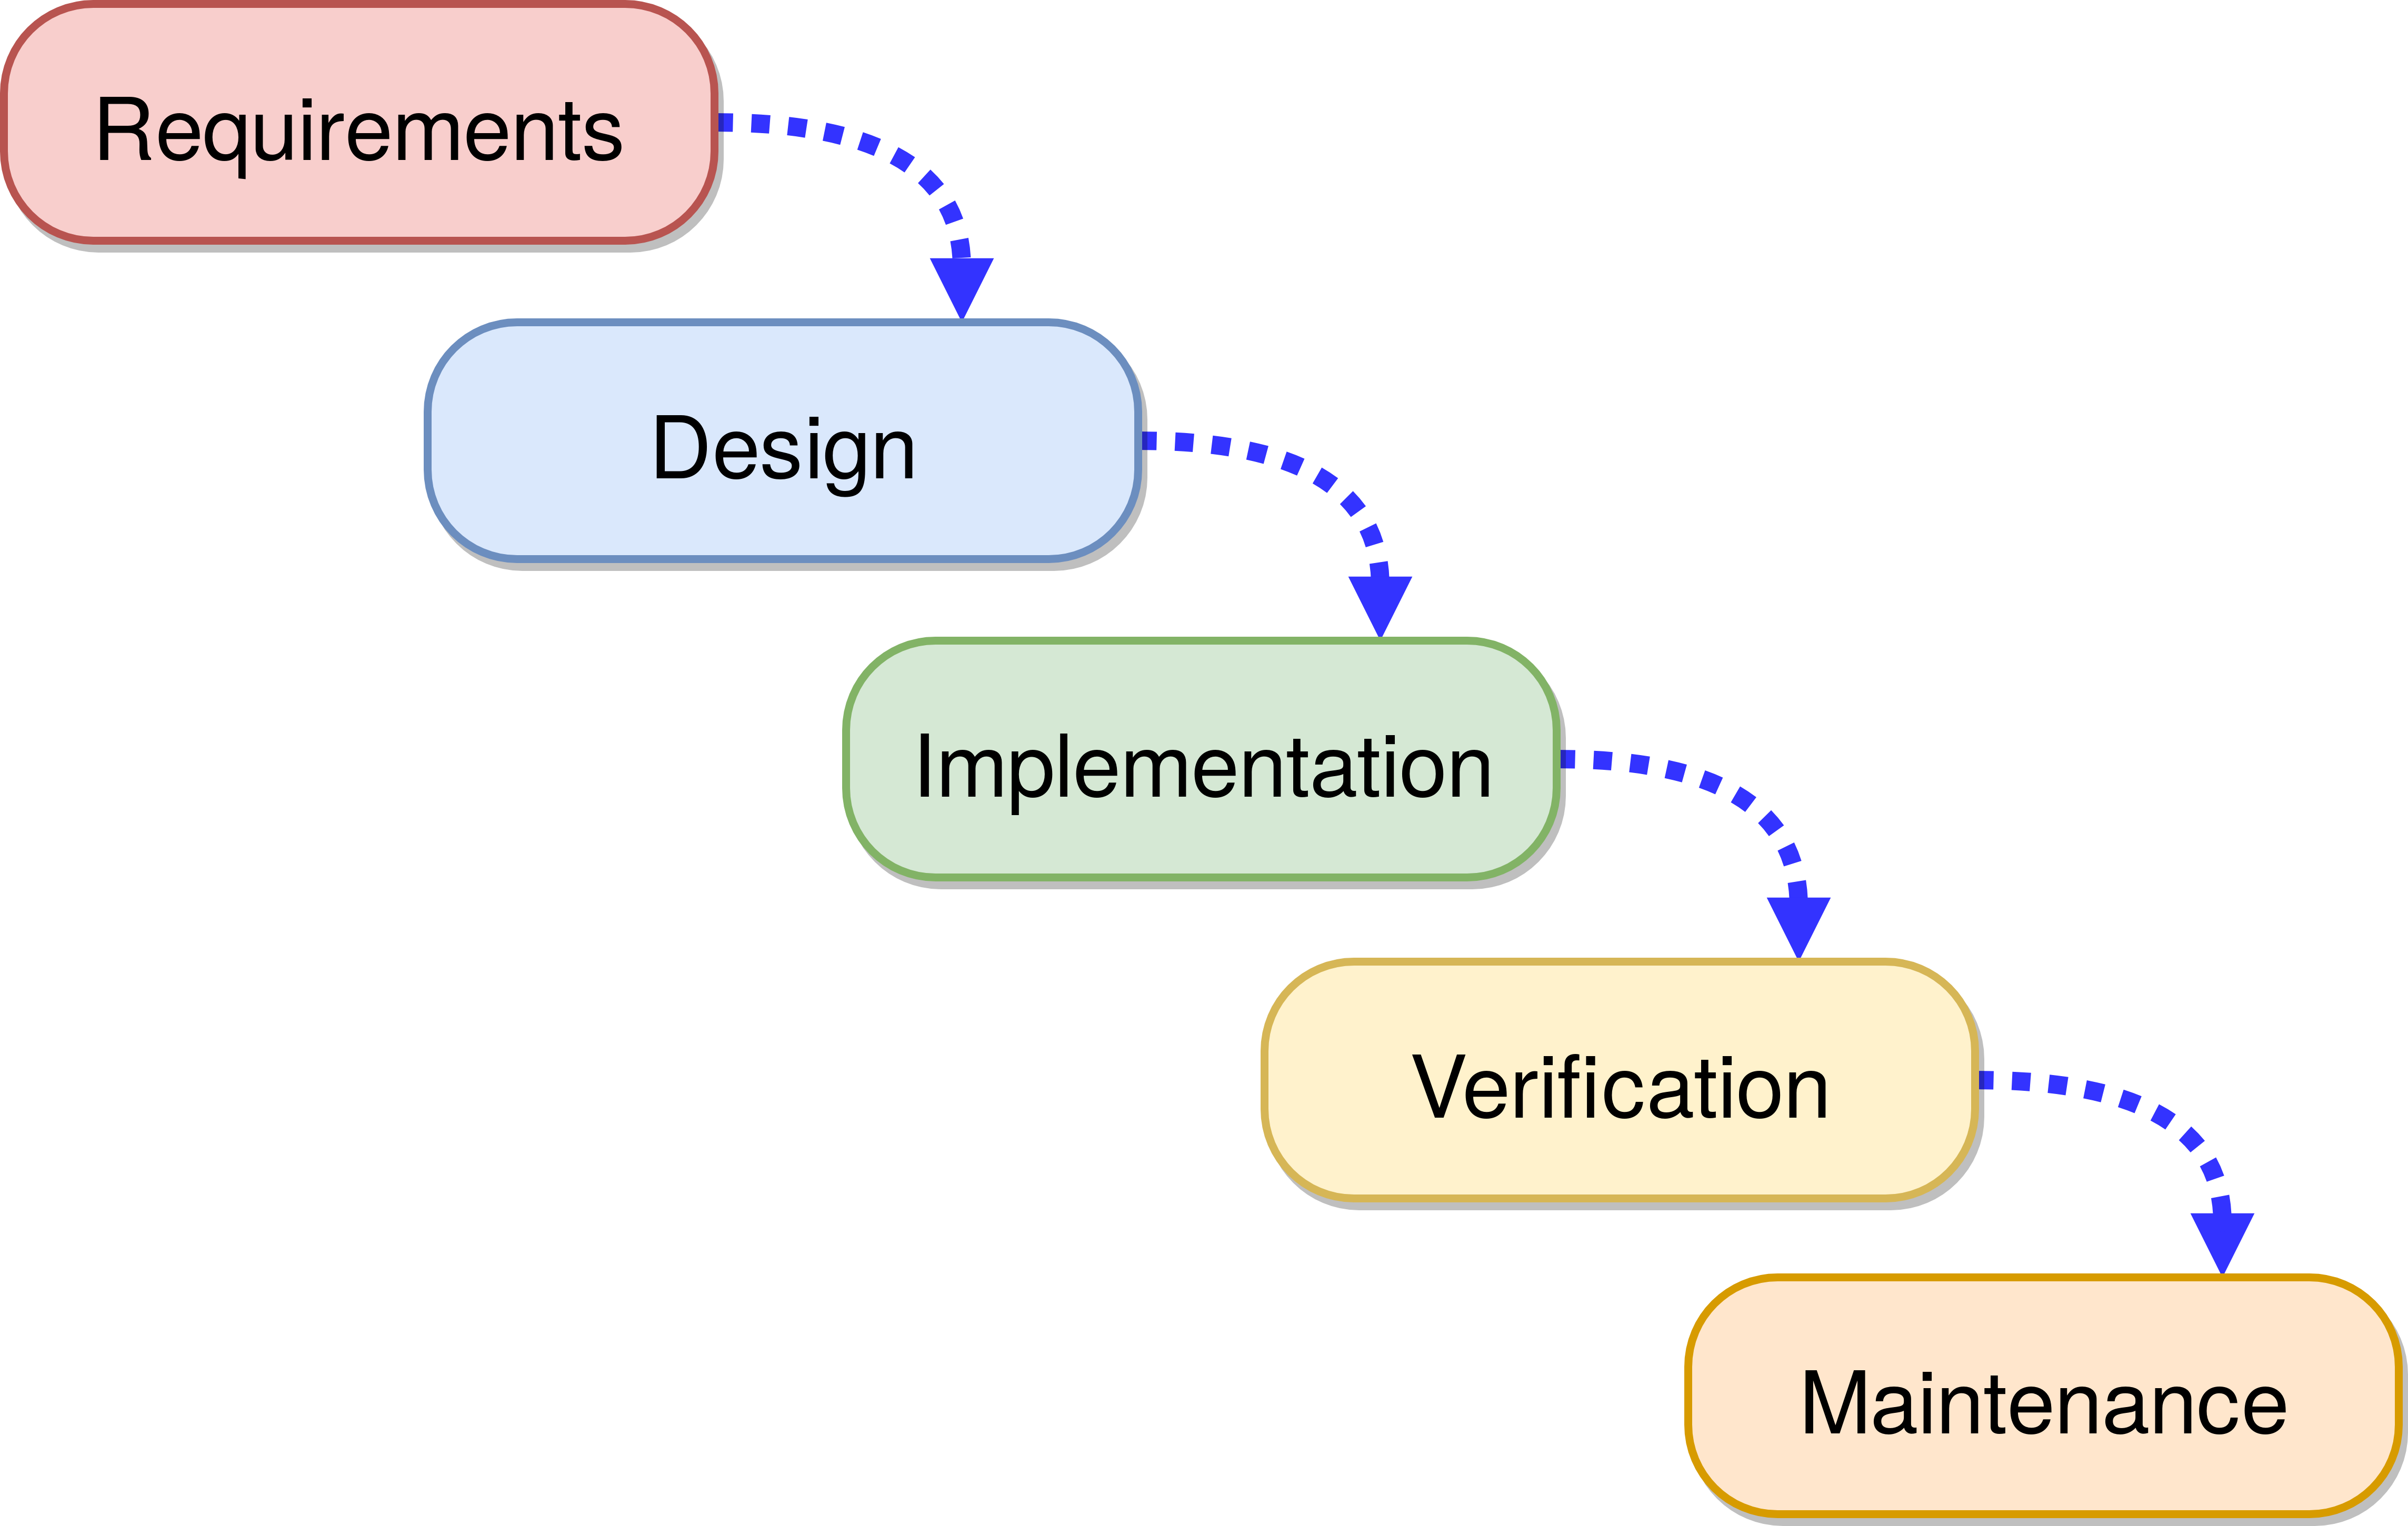
\includegraphics[width=0.75\textwidth]{../figures/waterfall_diagram.png}
\end{frame}

\begin{frame}
\frametitle{Software verification and validation}
\center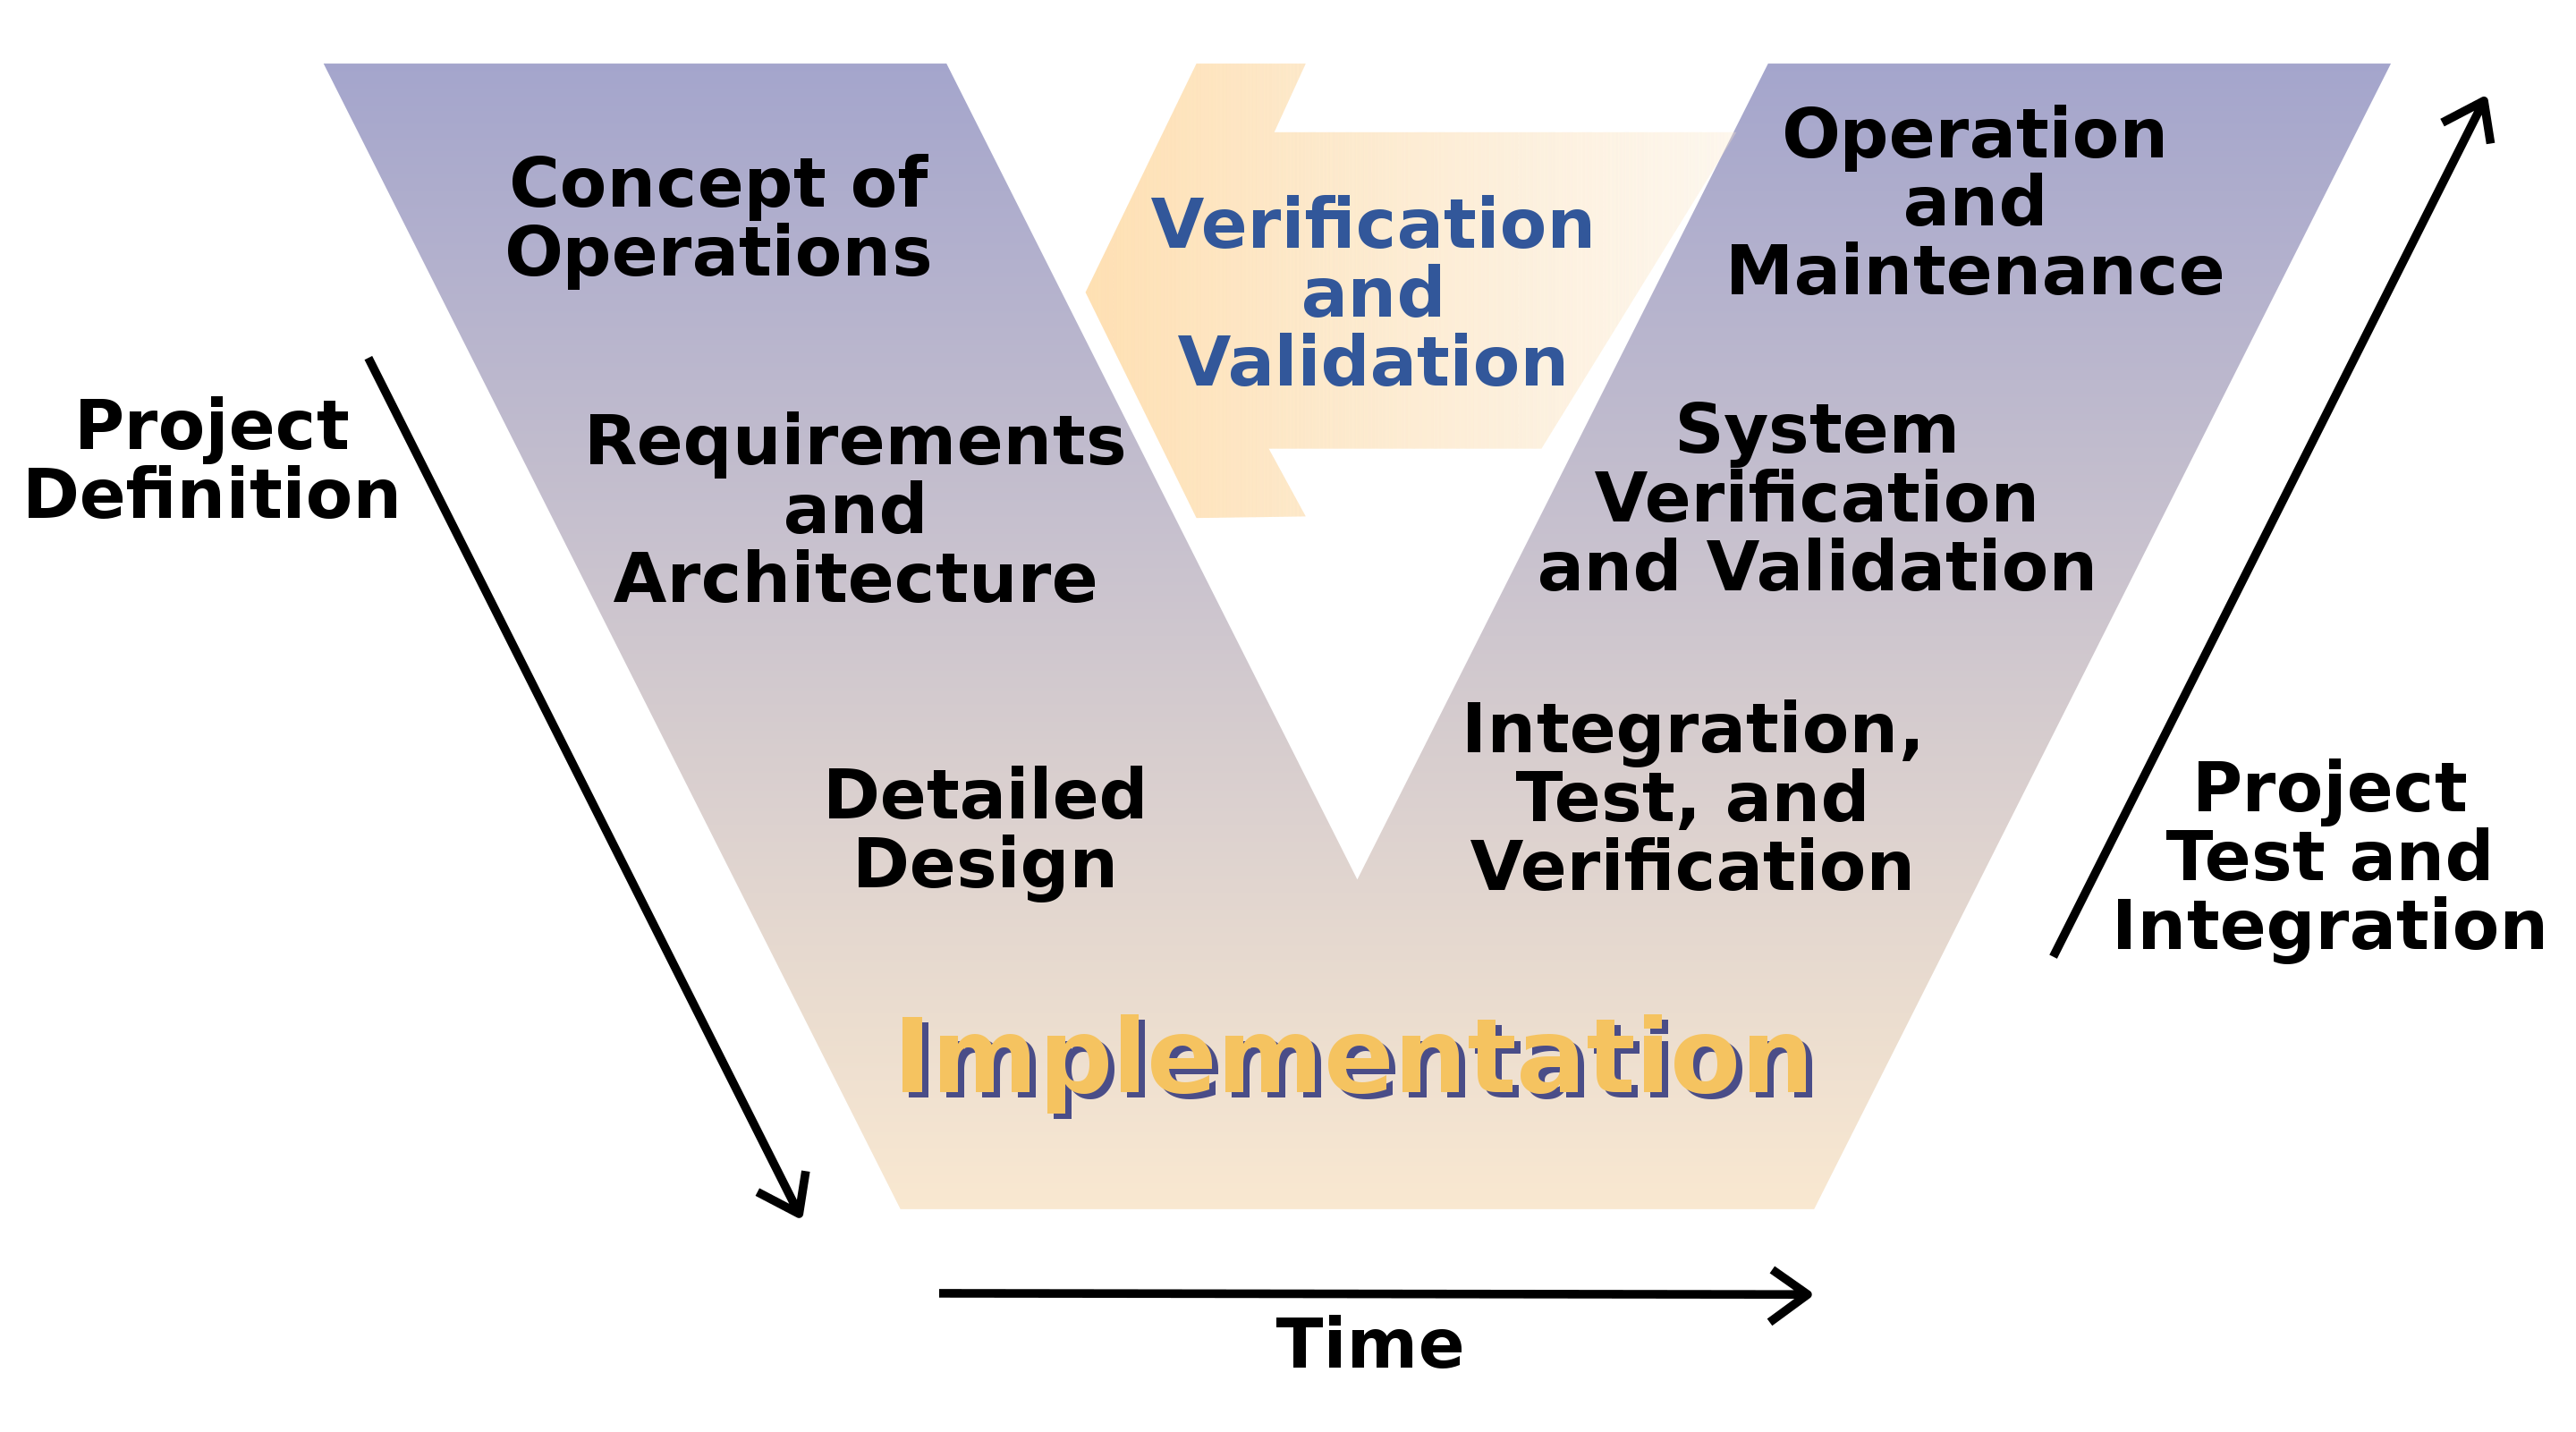
\includegraphics[width=0.75\textwidth]{../figures/verification_validation.png}
\end{frame}

\begin{frame}
\frametitle{Simple feedback systems}
\vspace{-0.8cm}
\center\scalebox{.5}{
\digraph{feedbackloop1}{
rankdir=LR;
node [fontname = "helvetica" shape=Mrecord style=filled];
layout="circo";
Decision -> Action -> Outcome -> Observation -> Choice -> Decision;
}
}
\end{frame}

\begin{frame}
\frametitle{Unmodeled dynamics}
\vspace{-0.8cm}
\center\scalebox{.5}{
\digraph{feedbackloop2}{
rankdir=LR;
node [fontname = "helvetica" shape=Mrecord style=filled];
layout="circo";
Decision -> Action -> Outcome -> Observation -> Choice -> Decision;
Eternalities[fillcolor=yellow];
Experience[fillcolor=yellow];
Perception[fillcolor=yellow];
Eternalities -> Outcome;
Experience -> Decision;
Perception -> Observation;
}
}
\end{frame}


%\begin{frame}
%\frametitle{Epistemic and Aleatoric Risk}
%
%\end{frame}

\begin{frame}
\frametitle{Closed loop control}
\center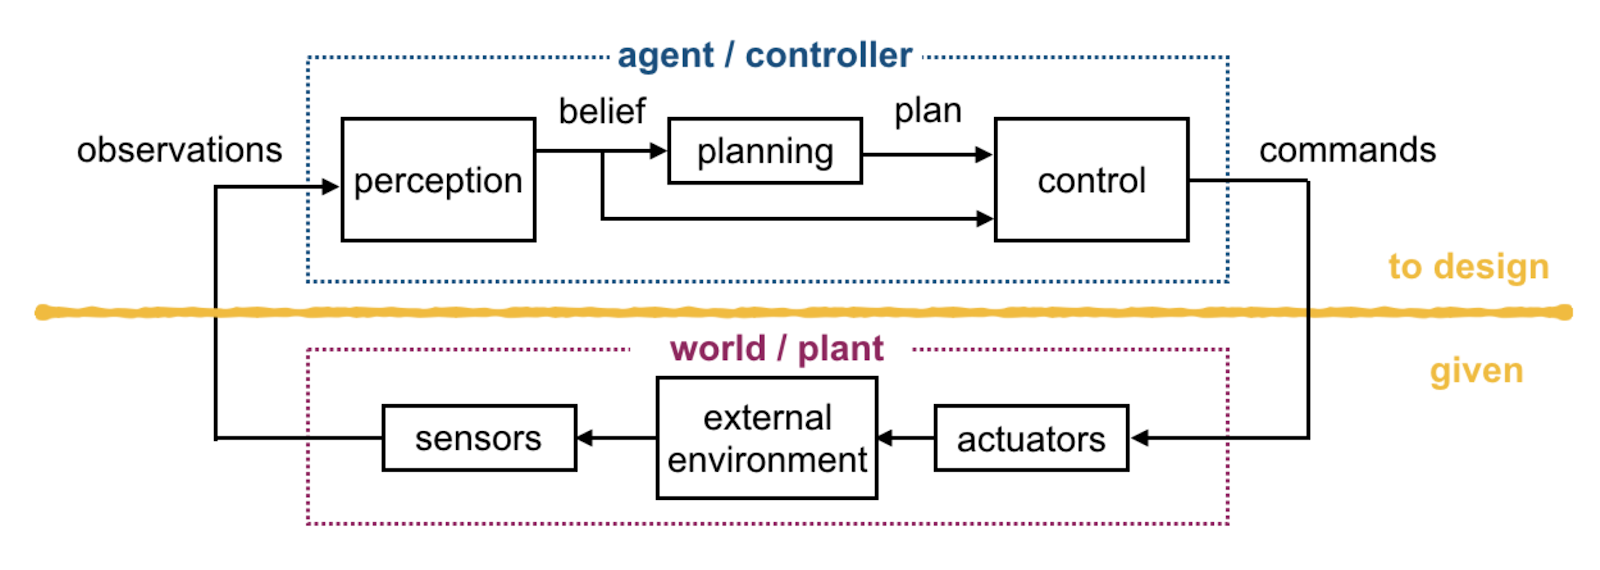
\includegraphics[width=0.85\textwidth]{../figures/agent_environment.png}

Where are the boundaries between these components? \\
How do we safely and effectively test these systems?
\end{frame}

\begin{frame}
\frametitle{Bias/Variance and Sensitivity/Specificity}
\center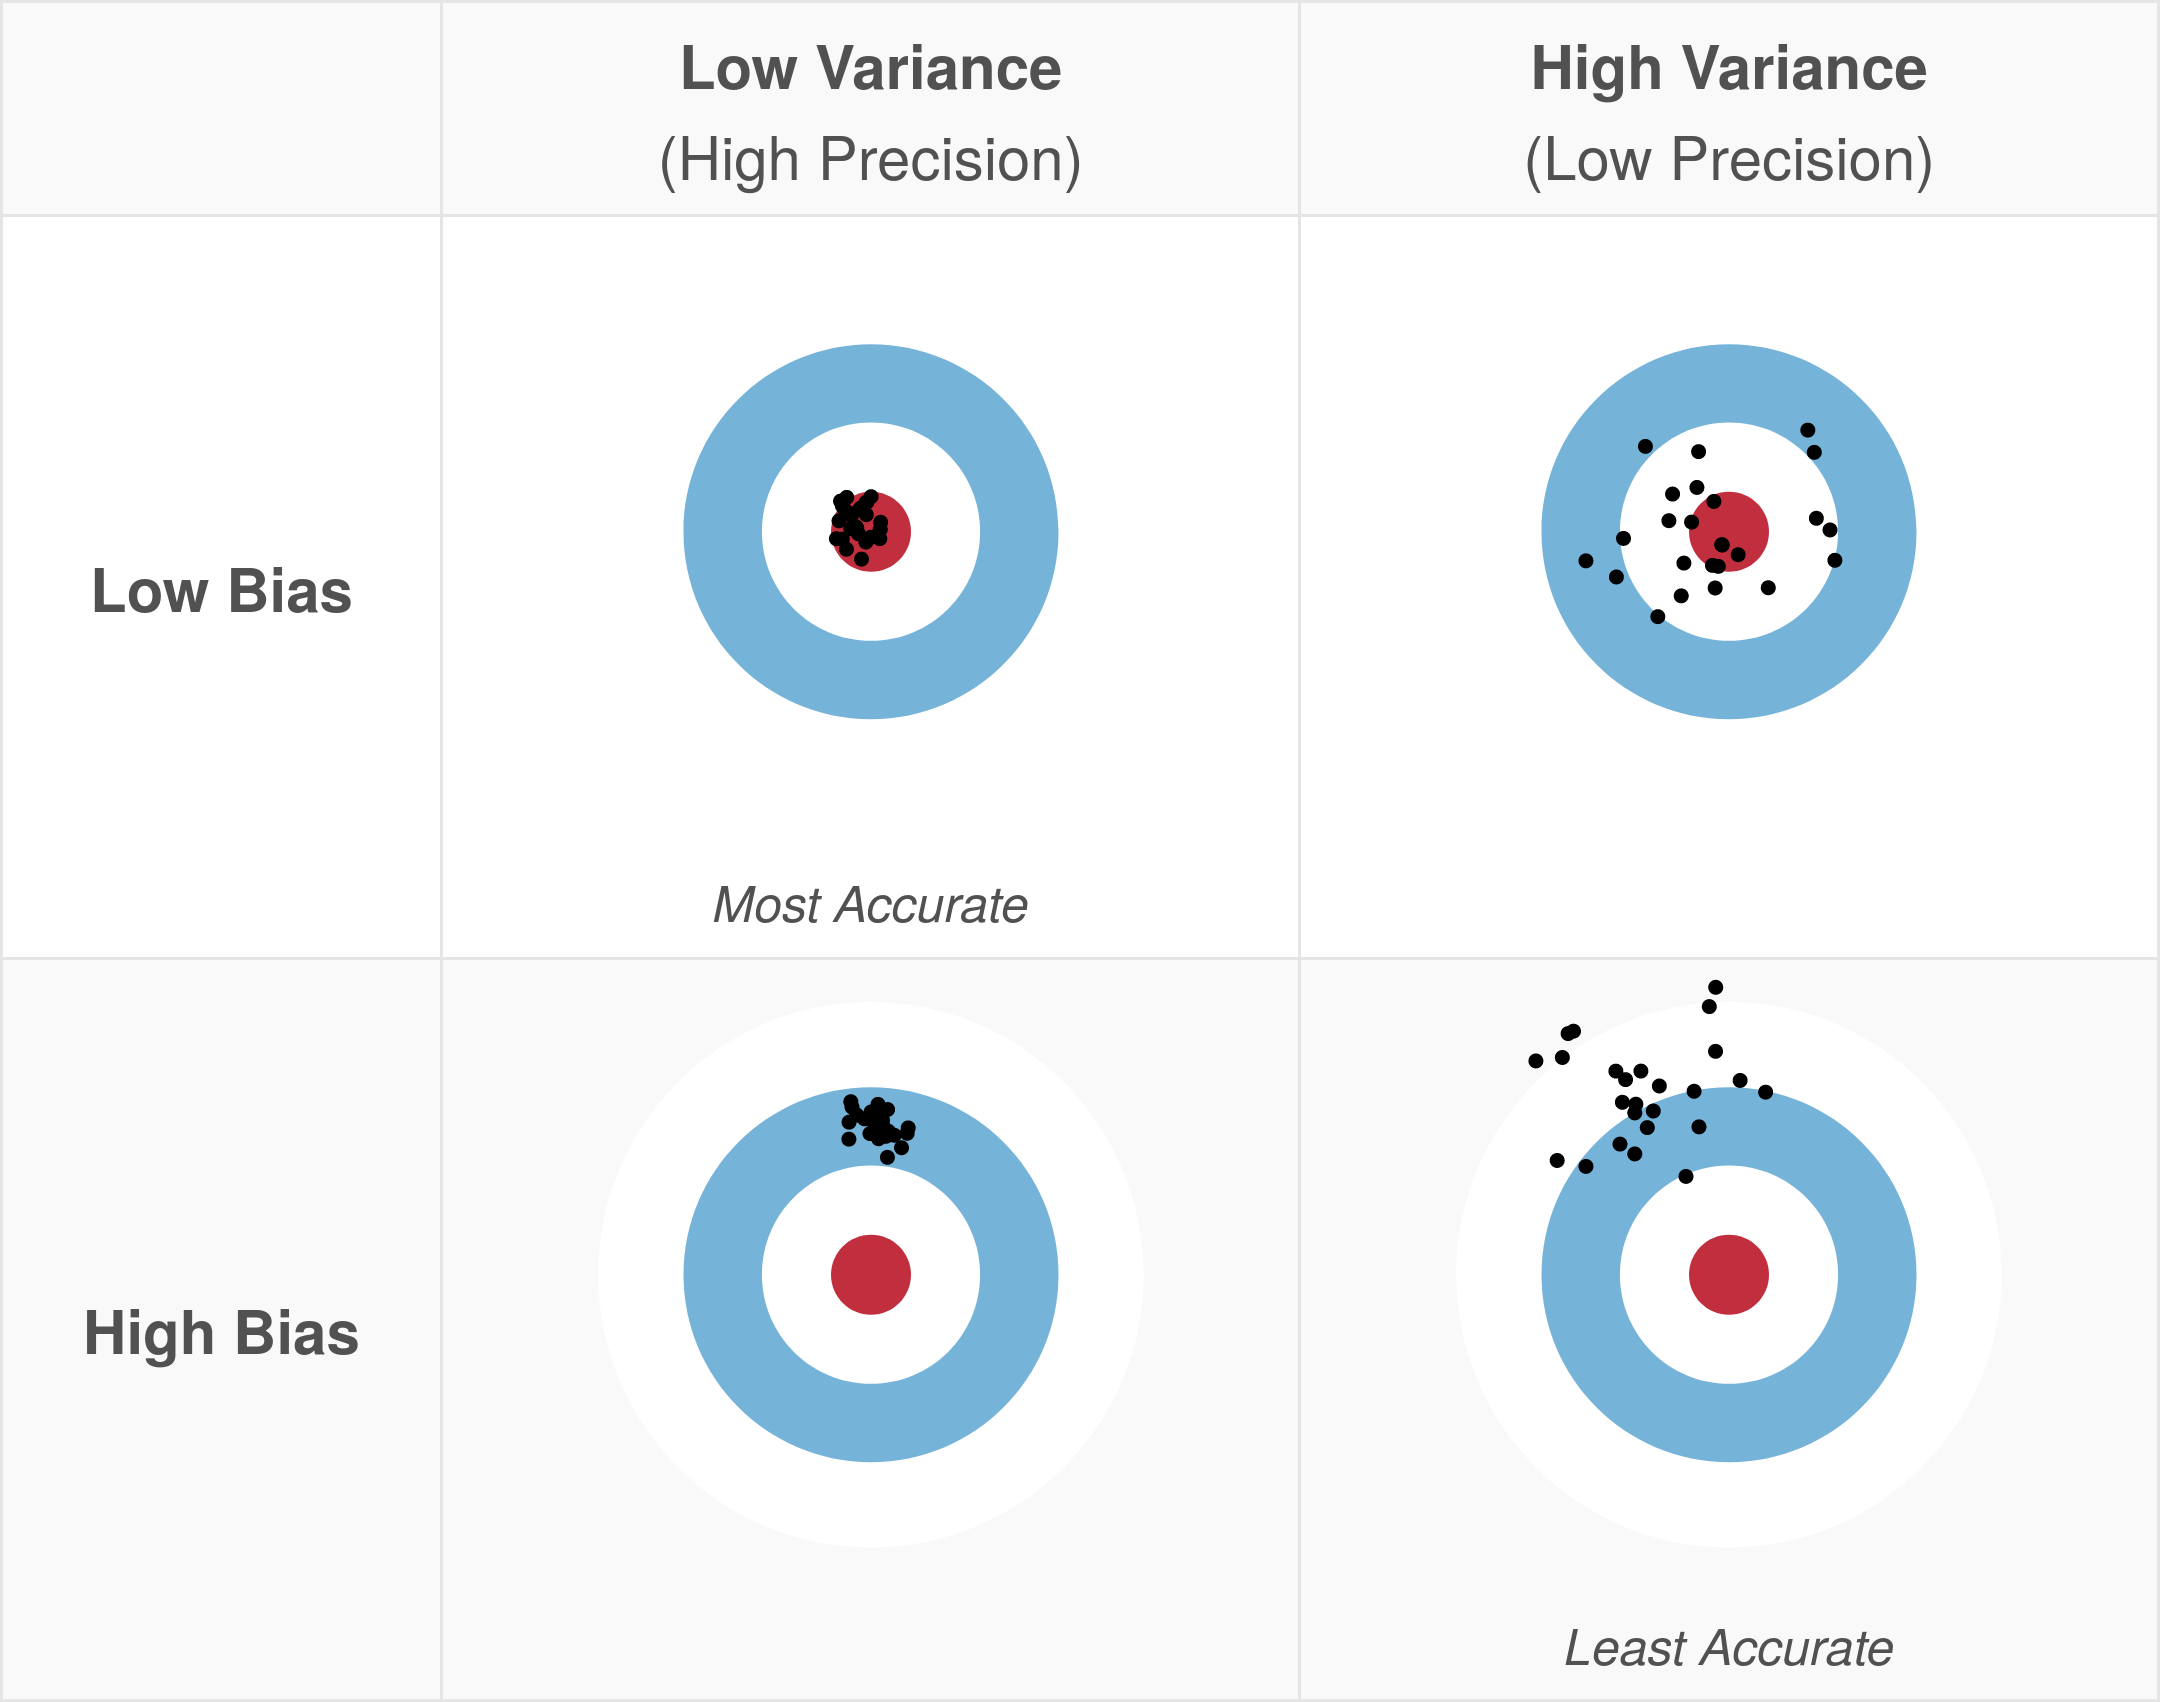
\includegraphics[width=0.70\textwidth]{../figures/bias_variance.png}
\end{frame}

\begin{frame}
\frametitle{Validity and testing}
\begin{enumerate}
\item Are we really measuring what we want to measure? (Test validity)
\begin{enumerate}
\item Many advertisers try to maximize clicks. This is a poor metric.
\item Objectives may change over the production lifetime of a model.
\item A poorly chosen objective can have unintended consequences.
\end{enumerate}
\item Is the dataset free from confounds? (Internal validity)
\begin{enumerate}
\item People constantly forget (or conveniently overlook) confounds.
\item If the data generator is biased, the model will encode its bias.
\item The method of sampling may have hidden biases.
\end{enumerate}
\item Does the model generalize well in practice? (External validity)
\begin{enumerate}
\item Maybe the training data has grown stale over time.
\item Maybe the model is missing data on some key demographic.
\item Maybe the true population is not the population we bargained for.
\end{enumerate}
\end{enumerate}
\end{frame}

\begin{frame}
\frametitle{Hypothesis Testing}
\vspace{-1cm}
\center\scalebox{.5}{
\digraph{hypotest}{
rankdir=TB;
node [fontname = "helvetica" width="2" shape=Mrecord style=filled];
"Formulate null and alternate hypotheses" -> "Determine statistical test and significance level" -> "Apply differential treatment" -> "Collect a sample, compare mean and variance" -> "Make a decision";
"Cannot reject null hypothesis"[fillcolor=yellow];
"Reject null, accept alternate"[fillcolor=green];
"Make a decision" -> "Cannot reject null hypothesis";
"Make a decision" -> "Reject null, accept alternate";
}
}
\end{frame}

\begin{frame}
\frametitle{Hypothesis Testing}
\center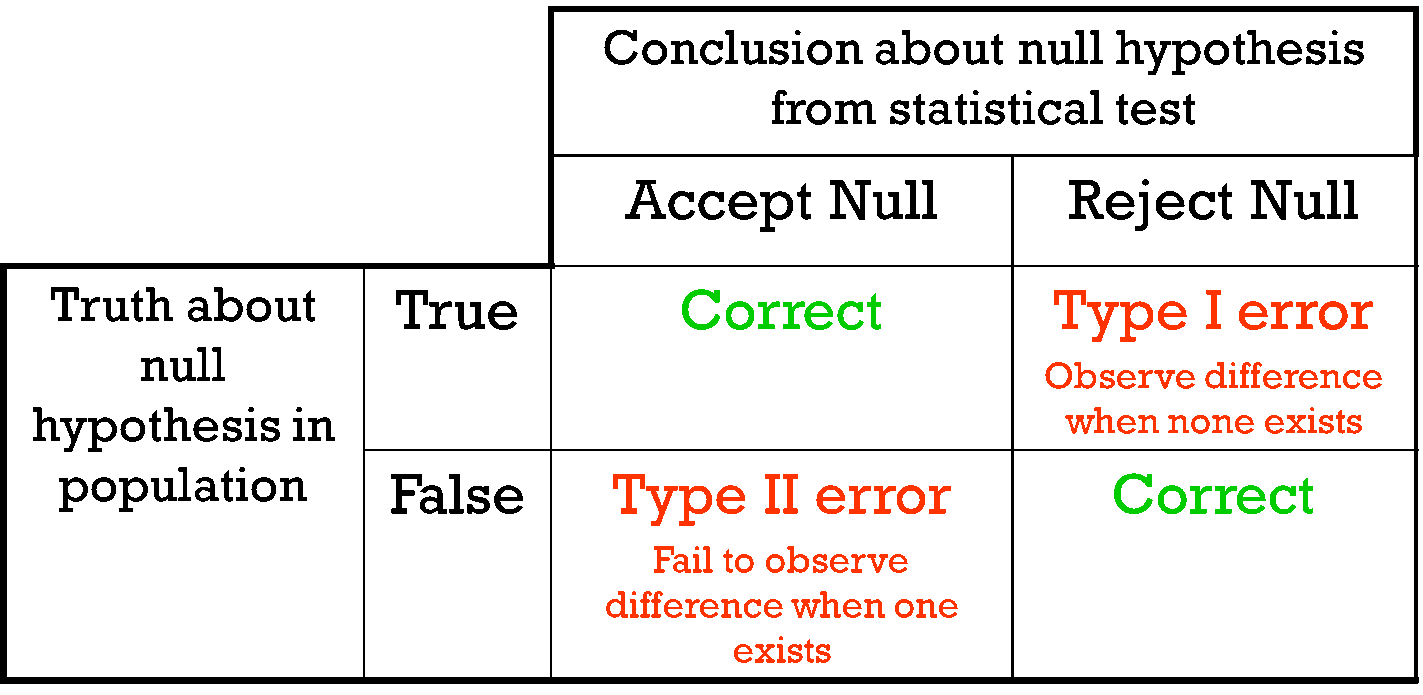
\includegraphics[width=0.85\textwidth]{../figures/hypothesis_testing.png}
\end{frame}

\begin{frame}
    \frametitle{A/B Testing}
    \center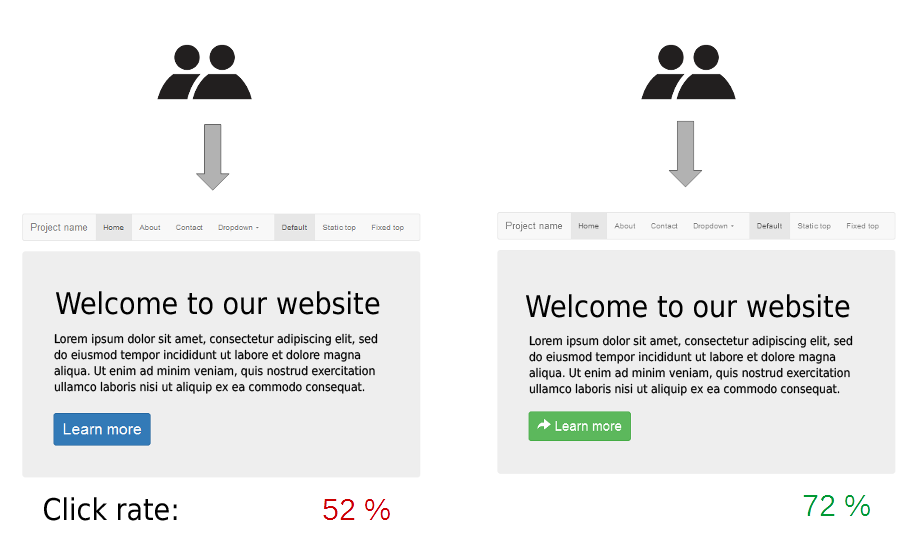
\includegraphics[width=0.85\textwidth]{../figures/ab_testing.png}
\end{frame}

\begin{frame}
    \frametitle{A/B Testing}
    \vspace{-1cm}
    \center\scalebox{.5}{
    \digraph{abtest}{
    rankdir=TB;
    node [fontname = "helvetica" width="2" shape=Mrecord style=filled];
    "Sees version A"[fillcolor=red];
    "Sees version B"[fillcolor=green];
    "Incoming user U" -> "Sample A/B from prior distribution" -> "Sees version A";
    "Sample A/B from prior distribution" -> "Sees version B";
    "Sees version A" -> "Measure engagement (e.g. clickthrough)";
    "Sees version B" -> "Measure engagement (e.g. clickthrough)";
    "Measure engagement (e.g. clickthrough)" -> "Evidence";
    "Evidence" -> "Update priors P(A|U), P(B|U)";
    }
    }
\end{frame}


\begin{frame}
    \frametitle{A/B/C Testing}
    \vspace{-1cm}
    \center\scalebox{.5}{
    \digraph{abctest}{
    rankdir=TB;
    node [fontname = "helvetica" width="2" shape=Mrecord style=filled];
    "Sees version A"[fillcolor=red];
    "Sees version B"[fillcolor=yellow];
    "Sees version C"[fillcolor=green];
    "Incoming user U" -> "Sample A/B/C from prior distribution" -> "Sees version A";
    "Sample A/B/C from prior distribution" -> "Sees version B";
    "Sample A/B/C from prior distribution" -> "Sees version C";
    "Sees version A" -> "Measure engagement (e.g. clickthrough)";
    "Sees version B" -> "Measure engagement (e.g. clickthrough)";
    "Sees version C" -> "Measure engagement (e.g. clickthrough)";
    "Measure engagement (e.g. clickthrough)" -> "Evidence";
    "Evidence" -> "Update priors P(A|U), P(B|U), P(C|U)";
    }
    }
\end{frame}


\begin{frame}
    \frametitle{Multi-armed bandits}
    \center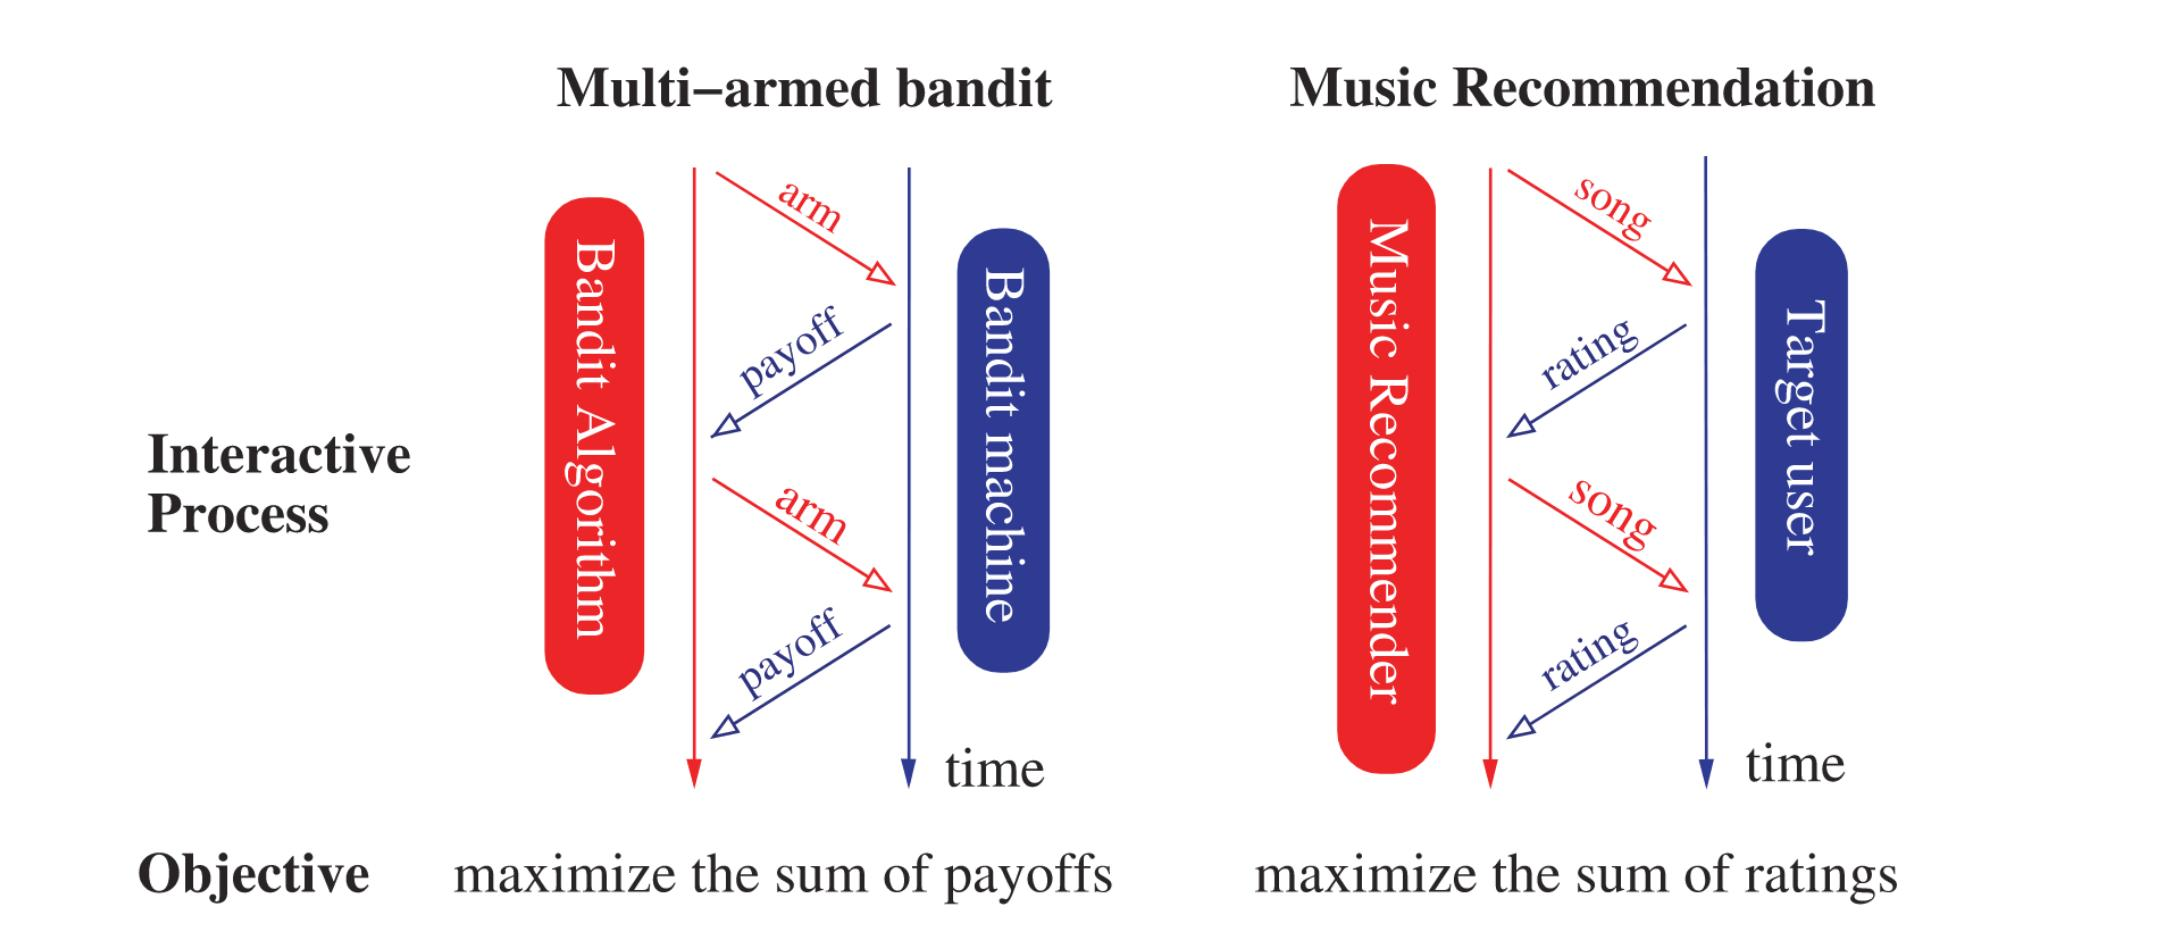
\includegraphics[width=0.95\textwidth]{../figures/mab_recommender.jpg}
    \url{https://dl.acm.org/doi/pdf/10.1145/2623372#page=8}
\end{frame}

\section{Software Testing Strategies}

\begin{frame}[fragile]
\frametitle{Unit Testing}
Checks a small ``unit'' of code on a small number of input/outputs.
\begin{kotlinlisting}
fun test(subroutine: (Input) -> Output) {
  val input = Input()           // Construct an input
  val expectedOutput = Output() // Construct an output
  val actualOutput = subroutine(input)
  assert(expectedOutput == actualOutput) { // Evaluate
    "Expected $expectedOutput, got $actualOutput"
  }
}
\end{kotlinlisting}
\textbf{Pros}: Simple to understand and helps document design assumptions.\\
\textbf{Cons}: High coverage is cumbersome to write, grows stale over time.
\end{frame}

\begin{frame}[fragile]
\frametitle{Integration Testing}
Checks for terminating exceptions and postconditions on a large program.
\begin{kotlinlisting}
fun <I, O> test(program: (I) -> O, inputs: Set<I>) =
  inputs.forEach { input: I ->
    try {
      val output: O = program(input) // Whole program
      assert(postcondition(output)) {
        "Postcondition failed on $input, $output"
      }
    } catch (exception: Exception) {
      assert(false) { exception }  //
    }
  }
\end{kotlinlisting}
\textbf{Pros}: Easier to write, checks for high-level exceptions and postconditions. \\
\textbf{Cons}: Only covers the ``happy path'', can often be too coarse grained.
\end{frame}

%\begin{frame}[fragile]
%\frametitle{Integration testing dataflow}
%\vspace{-1.5cm}
%\begin{kotlinlisting}
%fun <I, O> test(program: (I) -> O, inputs: Set<I>) =
%  inputs.forEach { input: I ->
%    try {
%      val output: O = program(input) // Whole program
%      assert(postcondition(output)) {
%        "Postcondition failed on input, output"
%      }
%    } catch (exception: Exception) { assert(false) }
%  }
%\end{kotlinlisting}
%\vspace{-2.5cm}
%\scalebox{.5}{
%\center\digraph{itestflow}{
%rankdir=LR;
%node [fontname = "helvetica" shape=Mrecord style=filled];
%Input -> Program -> Output -> "Postcondition?" -> Pass;
%"Postcondition?" -> Fail;
%Program -> Crash -> Fail;
%{rank = same; Crash Output }
%}
%}
%\end{frame}

\begin{frame}[fragile]
\frametitle{Fuzz Testing}
Generates many random inputs and compare outputs with an oracle.
\begin{kotlinlisting}
@Repeat(LARGE_NUMBER)
fun <I, O> test(program: (I) -> O, // System under test
                oracle : (I) -> O, // Source of Truth
                sample : (Random)  -> I) {
    val input: I = sample(Random())
    assert(program(input) == oracle(input)) {
      "Oracle and program disagree on $input"
    }
  }
\end{kotlinlisting}
\textbf{Pros}: Lower effort required to write test cases, higher test coverage. \\
\textbf{Cons}: Input space often too large to brute force, ``test oracle problem''.
\end{frame}
\begin{frame}[fragile]
\frametitle{Fuzzing Dataflow}
\vspace{-0.2}
\begin{kotlinlisting}
@Repeat(LARGE_NUMBER)
fun <I, O> test(program: (I) -> O, // System under test
                oracle : (I) -> O, // Source of Truth
                sample : (Random)  -> I) {
  val input: I = sample(Random())
  assert(program(input) == oracle(input)) {
    "Oracle and program disagree on $input"
  }
}
\end{kotlinlisting}
\center\scalebox{.5}{
\digraph{fuzzing}{
rankdir=LR;
node [fontname = "helvetica" shape=Mrecord style=filled];
Random -> Sample;
Sample -> Input;
Input -> Program -> Output;
Input -> Oracle -> Answer;
{rank = same; Program Oracle }
Output -> "Same?";
Answer -> "Same?";
{rank = same; Output Answer }
}
}
\end{frame}


\begin{frame}[fragile]
\frametitle{Property Based Testing}
Specify a universal output property and implement a sampler and shrinker.
\begin{kotlinlisting}
@Repeat(LARGE_NUMBER)
fun <I, O> test(program : (I) -> O,
                property: (O) -> Boolean,
                sample  : (Random) -> I,
                shrinker: (I, (I)->O, (O)->Boolean) -> I) {
    val randomInput: I = sample(Random())
    assert(property(program(randomInput))) {
      "Error detected on: $randomInput!"
      val min = shrinker(randomInput, program, property)
      "Minimal counterexample of property: $min!"
    }
  }
\end{kotlinlisting}
\textbf{Pros}: No oracle required, can detect and minimize counterexamples. \\
\textbf{Cons}: Property specification can be brittle and requires domain expertise.
\end{frame}


\begin{frame}[fragile]
\frametitle{PBT Dataflow}
\begin{kotlinlisting}
@Repeat(LARGE_NUMBER)
fun <I, O> test(program : (I) -> O,
                property: (O) -> Boolean,
                sample  : (Random) -> I,
                shrinker: (I, (I)->O, (O)->Boolean) -> I) {
  val randomInput: I = sample(Random())
  assert(property(program(randomInput))) {
    "Error detected on: $randomInput!"
    val min = shrinker(randomInput, program, property)
    "Minimal counterexample of property: $min!"
  }
}
\end{kotlinlisting}
\vspace{-1.5cm}
\center\scalebox{.5}{
\digraph{pbtflow}{
rankdir=LR;
node [fontname = "helvetica" shape=Mrecord style=filled];
Random -> Sample -> Input -> Program -> "Property?" -> Shrinker -> Input;
}
}
\end{frame}


\begin{frame}[fragile]
\frametitle{Metamorphic Testing}
Specify a relation (e.g. $\approx$), transform inputs and compare with labels.
\begin{kotlinlisting}
@Repeat(LARGE_NUMBER)
fun <I, O> test(program: (I)               -> O,
                inputTx: (I)               -> I,
                metaRel: (O, O)            -> Boolean,
                sample : (Set<Pair<I, O>>) -> Pair<I, O>,
                dataset: Set<Pair<I, O>>) {
    val (trueInput: I, trueOutput: O) = sample(dataset)
    val transformedInput : I = inputTx(input)
    val transformedOutput: O = program(transformedInput)
    assert(metaRel(trueOutput, transformedOutput)) {
      "<$trueOutput> not $metaRel <$transformedOutput>!"
    }
  }
\end{kotlinlisting}
\textbf{Pros}: No domain expertise required, just a small labeled dataset.\\
\textbf{Cons}: How to design TX to detect errors efficiently? Open research.
\end{frame}


\begin{frame}[fragile]
\frametitle{MMT Dataflow}
\vspace{-0.2cm}
\begin{kotlinlisting}
@Repeat(LARGE_NUMBER)
fun <I, O> test(program: (I)               -> O,
                inputTx: (I)               -> I,
                metaRel: (O, O)            -> Boolean,
                sample : (Set<Pair<I, O>>) -> Pair<I, O>,
                dataset: Set<Pair<I, O>>) {
    val (trueInput: I, trueOutput: O) = sample(dataset)
    val transformedInput : I = inputTx(input)
    val transformedOutput: O = program(transformedInput)
    assert(metaRel(trueOutput, transformedOutput)) {
      "<$trueOutput> not $metaRel <$transformedOutput>!"
    }
  }
\end{kotlinlisting}
\vspace{-1.5cm}
\center\scalebox{.5}{
\digraph{metamorphic}{
rankdir=LR;
node [fontname = "helvetica" shape=Mrecord style=filled];
Dataset -> Sample;
Sample -> Input;
Sample -> Label;
{rank = same; Input Label }
Input -> Transform -> Program;
Program -> "MR?";
Label -> "MR?";
}
}
\end{frame}

\begin{frame}
\frametitle{Hypothesis testing vs. Software testing}
\begin{multicols}{2}
\underline{Statistical Testing}
\begin{itemize}
\item We're not sure what the correct answer is, want to find out
\item Tries to minimize empirical risk by increasing sample size
\item Often assumes IID randomness for accurate results
\item Deliberately injects noise into sampling process
\item Results are never exactly the same twice
\item Requires non-determinism to demonstrate reproducibility
\end{itemize}
\vfill\null
\columnbreak
\underline{Software Testing}
\begin{itemize}
\item We know what the correct behavior is, need to validate it!
\item Tries to minimize operational risk, increase test coverage
\item Uses randomness as a substitute for formal verification
\item Tries to reduce noise to prevent false alarms
\item Requires determinism for software reproducibility
\end{itemize}
\end{multicols}
\end{frame}


% \begin{frame}
% \frametitle{Statistical vs. Systematic uncertainty}
%
% \end{frame}

\begin{frame}
\frametitle{Further resources}
\begin{enumerate}
\item \href{https://arxiv.org/pdf/1910.09457.pdf}{Aleatoric and Epistemic Uncertainty in Machine Learning}, Eyke H\"ullermeieraand Willem Waegeman (2020)
\item \href{https://lilianweng.github.io/lil-log/2018/01/23/the-multi-armed-bandit-problem-and-its-solutions.html#thompson-sampling}{The Multi-Armed Bandit Problem and Its Solutions}, Weng (2017)
\item \href{https://dl.acm.org/doi/pdf/10.1145/2623372}{Exploration in Interactive Music Recommendation}, Wang (2014)
\item \href{https://alexwlchan.net/2016/06/hypothesis-intro/}{Intro to property-based testing}, Alex Chan (2016)
\item \href{https://felginep.github.io/2019-03-20/property-based-testing}{Property based testing}, Pierre Felgines (2019)
\item \href{https://lemonidas.github.io/pdf/FuzzChick.pdf}{Coverage Guided, Property Based Testing}, Lamproproulos (2019)
\item \href{https://www.hillelwayne.com/post/metamorphic-testing/}{Metamorphic testing}, Wayne (2019)
\item \href{https://mcminn.io/publications/tr3.pdf}{Survey of Trends in Oracles for Software Testing}, Harman (2014)
\item \href{https://lcamtuf.coredump.cx/afl/}{American Fuzzy Lop}
\item \href{http://proceedings.mlr.press/v97/odena19a/odena19a.pdf}{TensorFuzz: Debugging Neural Networks with Coverage-Guided Fuzzing}, Odena et al. (2019)
\end{enumerate}
\end{frame}

\end{document}